\begin{center}
Dusty 'Star Colonel' Guerra
\end{center}

\ifthenelse{\not \equal{\outworldsMode}{mode-web}}{\begin{multicols}{2}}{}

\emph{
\bfseries
\\Braizo Plains\\
\noindent
Renorsal, Outworlds Wastes\\
15 November 3064
}

Blinding blue-white beams lashed across the wind swept, barren landscape of the Braizo Plains.
One particle bolt slammed into rock outcropping, filling the air with splintered stone shards as the rock exploded under the hellish forces.

Through the shower of rock and dust, the second beam drilled into the barrel-chest of a \emph{Wolverine}.
Wherever the PPC beam touched it eviscerated the ferro-fibrous armor, seeking to punch through to the vital inner workings beneath.

Riding in the cockpit of her \emph{Ice Ferret}, Sandra cast a glance at Kamran's \emph{Warhawk} stalking along a ridge behind her.
The assault OmniMech vented heat in the rear display over her primary holographic as its pilot relocated the massive weapons platform.

Undaunted by the strike despite the damage, the \emph{Wolverine} pilot unleashed a double burst of suppressing autocannon fire as he jumped for better cover.

"Seeker Three," Star Commander Malik Kirov's voice growled over the comms. "Swing wide to the left and move around their flank."

"\emph{Aff}, Seeker Lead."

Channeling her sense of balance into the neural link, Sandra leaned her forty-five ton war machine left as she altered course.

\emph{
Malik warned his vision promised conflict.
Yet it will be a small price to pay to discover the fate of the 61\textsuperscript{st} Royal Jump Infantry.
That so many other groups are on this world, seemingly searching for something, is a strong indicator that Malik is correct.
}

\emph{
Groups like these mercenaries{\ldots}
}

Sandra darted the \emph{Ice Ferret} through a narrow gap in another rock formation then burst into the open, throwing her OmniMech into a 129 kph sprint. 

\vspace{-3pt}
\par\noindent\centerline{\rule{0.4\columnwidth}{1pt}}

"Charlie will you watch where you're going?!"

The Demolisher assault tank tilted dangerously as the left side treads rolled up and over a boulder.
Twin Gauss Rifle barrels, adorned with the words 'Diplomacy Failed' scrawled on them in white, nearly scraped the ground as the gunner swung them back into line with the hull.

Used to this approach to driving, the crew wedged feet and arms against support structures to keep in their positions.

Despite Sergeant Dwight Shelby's complaints, Charles Harper knew he didn't care about the driving. He was griping to gripe.

It took the edge off driving a barely mobile tank into combat with the Clans.

"Diplomacy's a tank, Sarge, not a sports car."

"You could TRY not to hit every terrain feature," Gunner Austin Lane remarked over the comms. "Just a thought."

"You wanna drive, Aus?"

"No," Shelby cut off the chance for Austin to reply.
"We go through enough tracks without letting the kid with no license drive."

The tank rattled and slid sideways across loose scree as Charles manhandled it onto course, eliciting more curses.

"Shucks, Sarge," Charles remarked through gritted teeth. "I don't have a license neither."

"Contact! Look sharp!"

\vspace{-3pt}
\par\noindent\centerline{\rule{0.4\columnwidth}{1pt}}

Sandra's first warning was an urgent tone from her sensors.
A hostile contact flashed into existence on her holographic as the Demolisher seemed to materialize on the ridge just over three hundred meters away.
 
Yet again, the Goliath Scorpion warrior cursed the mineral deposits on world that had played hell with sensor operations since they landed.

Battle reflexes, bred into the Trueborn warrior through the advanced genetics programs of the Clans then honed to perfection, meant Sandra was evading the moment she was aware of the enemy tank.

It was still not fast enough.

The silvery blur of a Gauss Rifle hurtled across the desert to slam into the left arm of the \emph{Ice Ferret}.

Sandra wrestled with the controls, keeping the war machine upright by a combination of skill and determination.
Her eyes flashed to the damage indicator as it dutifully updated the condition of her OmniMech.

Internal structure damage on the arm, but no loss of functionality{\ldots}yet. Still, cannot take another hit like that!

The clan warrior ducked her machine behind a low ridge, breaking line of sight with the massive assault tank.

\emph{
Let's see how good your really are, \emph{surat}.
}

\vspace{-3pt}
\par\noindent\centerline{\rule{0.4\columnwidth}{1pt}}

"Hell yeah! Nice shootin' Lane!"

Charles couldn't help but grin at Shelby's words. 
It had been a hell of a shot to tag that \emph{Fenris} just as it exited the canyon.

\emph{
Not bad for a bunch of farm kids in an oversized tin can.
}

But now the tough part would really begin.
Already, Charles was shifting the controls to turn the ponderous tank.
It rarely benefited them to stay in the same position for long{\ldots}and he suspected it would be a matter of time before the inevitable happened.

Even anticipating it, he was surprised when it happened.

The \emph{Fenris} reemerged around the rock formation, running at a full sprint.
In mere seconds it chewed up the distance between itself and the ridge where Charles was trying to get Diplomacy into a better firing position.

Only thirty meters away, a defile would provide some cover for the tank while it continued to hurl Gauss rounds downrange.

Unfortunately, Diplomacy never got the chance to use it.

A quartet of stuttering emerald beams lashed out from the OmniMech, stabbing into the front and side of the turning armored vehicle.
Armor vaporized at the caress of pulse lasers and Diplomacy developed an unsettling and all too familiar grinding sound.

Charles cursed as the display in front of him flared a warning in red.

"We lost a track!"

There was a collective groan through the tank, audible over the engine and the discharge of twin Gauss Rifles overhead.

\vspace{-3pt}
\par\noindent\centerline{\rule{0.4\columnwidth}{1pt}}

One Gauss Rifle round tore past the cockpit of the \emph{Ice Ferret} so close Sandra thought she could feel the shock of its displacement through the air.
The other skipped off the ground to the OmniMechs right and ricocheted into its right thigh, sending a shudder through the war machine.

Once again, Sandra's skilled hand on the controls kept the ‘Mech upright but she gritted her teeth noting half the armor on the leg was gone.
Grudgingly, she acknowledged the skill of the tank's gunner.

\emph{
But it is all coming to an end now.
}

Smoke drifted up from the hull of the now immobilized tank.
Magnification confirmed the OmniMech's battle computer report; the tank had lost its left track.

It was little more than a pillbox.
A thickly armored and well-armed pillbox, but still an immobile target.

Planting one foot, Sandra leaned her ‘Mech so hard to the right she could have placed a hand on the ground as she reversed the OmniMech's course to rush right at the tank.

Feeling the shot more than aiming, she lashed the enemy tank with more pulse laser fire.
Only two connected and neither did more than damage more armor, of which the machine seemed to have an endless supply.

Now, however, the mercenary tank brought back up weapons online.
A pair of medium lasers returned her fire, cutting protection from the left flank and centerline of the OmniMech.
It was not enough to punch through, but it softened the war machine up should another Gauss Rifle round find its mark.

\emph{
You are a bruiser for certain{\ldots}but let us try something unorthodox, \emph{quiaff}?
}

\vspace{-3pt}
\par\noindent\centerline{\rule{0.4\columnwidth}{1pt}}

"Austin will you tag that damn thing already!"

Shelby coughed as smoke drifted through the compartment of Diplomacy, courtesy of a shorted-out display.
The tanks turret ground right as Austin tried to track the fast-moving OmniMech.

"You wanna convince the damn Clanner to stop moving so I can?"

Charles squinted through the viewport, watching the \emph{Fenris} change course.
It was one of the sharpest bits of ‘Mech piloting he'd seen outside that pirated copy of last year's Noisel Summer Games.

"He's coming right at us," he called to the gunner. "Make it count, Aus!"

\ifthenelse{\not \equal{\outworldsMode}{mode-web}}{\end{multicols}}{}

\newpage

\subsection{Firefight}

\begin{figure}[!h]
  \centering
  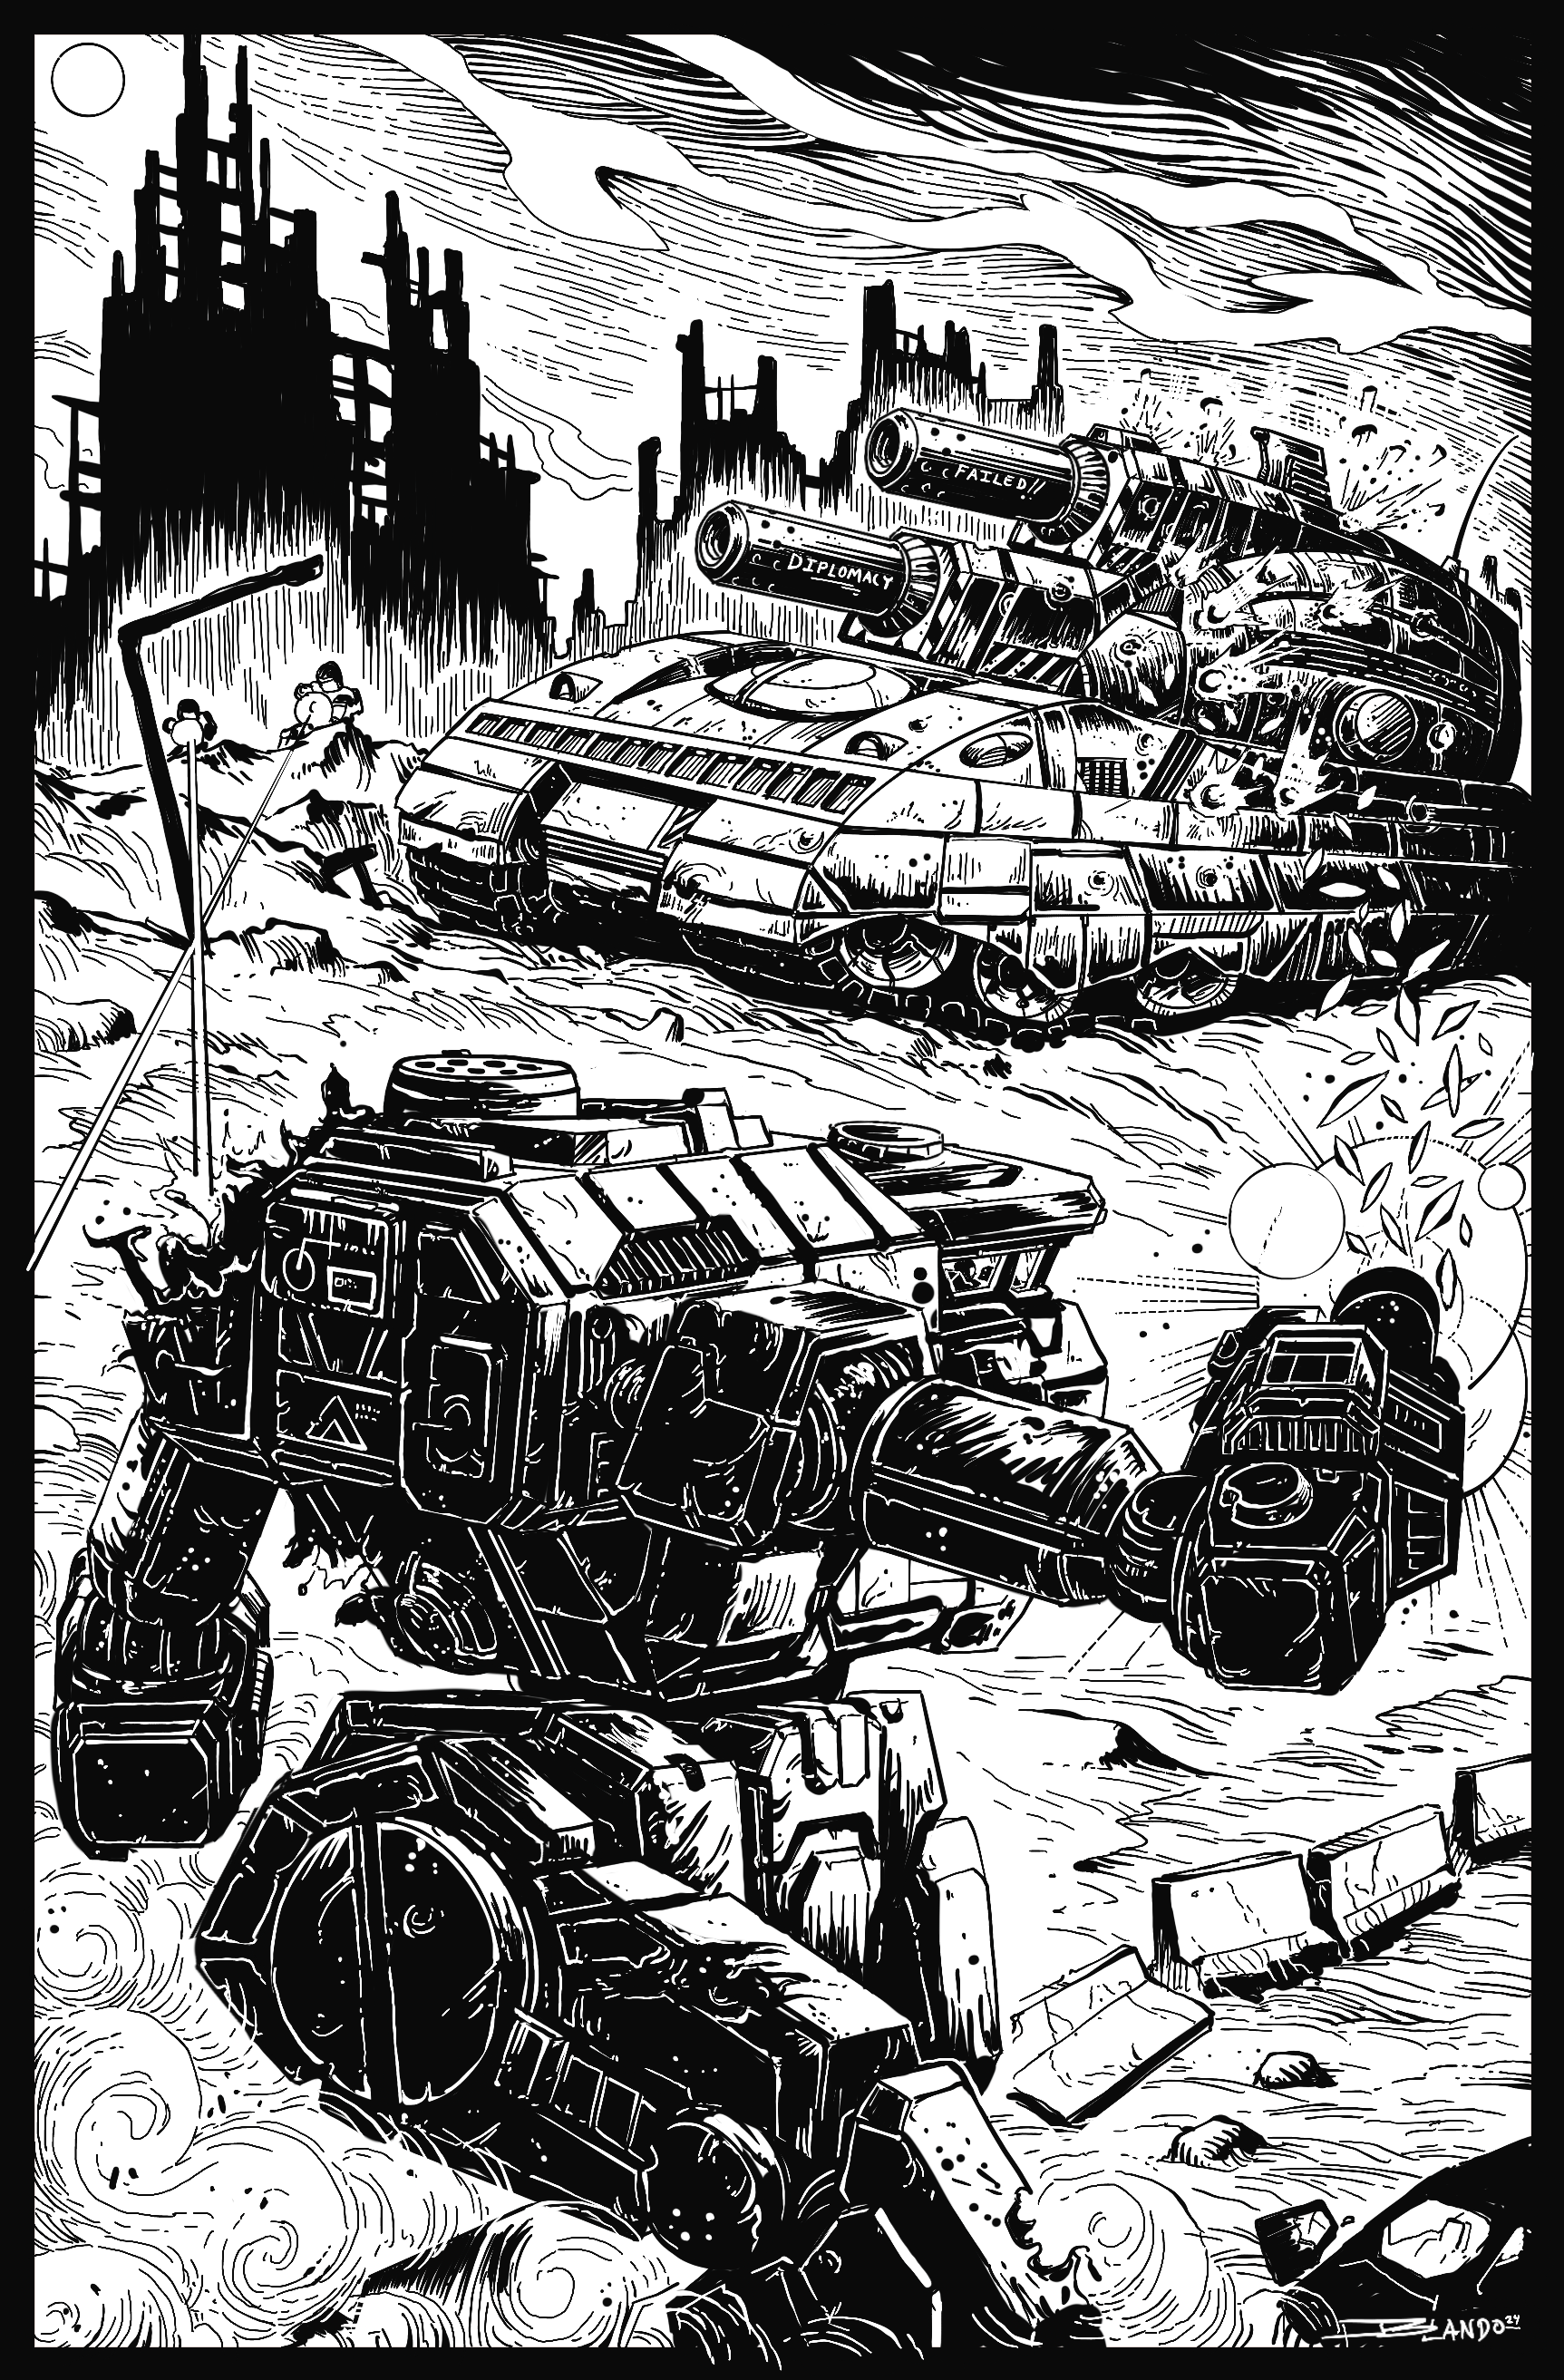
\includegraphics[alt='Demolisher and Ice Ferret fighting', width=5.5in, height=8.5in]{img/Firefight.png}
  \caption*{Firefight between \emph{Diplomacy Failed} and \emph{Ice Ferret} - \href{https://jaredblando.com/}{Jared Blando}}
\end{figure}

\newpage

\ifthenelse{\not \equal{\outworldsMode}{mode-web}}{\begin{multicols}{2}}{}

Another Gauss round slammed into the right torso of the \emph{Ice Ferret}, smashing armor and cracking the internal structure.
Warnings flashed indicating the frame of the war machine had taken damage and another hit there would likely damage the fusion reactor.

Sandra kept her OmniMech on course, determined to end this struggle one way or another.
Lasers flashed at her but both missed as she sidestepped the \emph{Ice Ferret} around a low hill then raced up to the tank.

The first kick crashed into the side of the armored vehicle, denting armor and crushing a pair of boggie wheels.
It was a testament to the design of the Demolisher that the plating held up under the assault of a 45-ton ‘Mech.

Undoubtedly, the crew was rattled when Sandra delivered a second kick in rapid succession.

\emph{
You all assume we do not know how to fight in close, Sandra grinned.
But in the 3\textsuperscript{rd} Cuirassiers, it is a point of pride.
}

The armor cracked under the assault and the OmniMech battle computer indicated there was a chance of internal damage.
Another strike there, lasers or a kick, would likely destroy the enemy tank.

"All Seekers," Malik's voice cut through Sandra's cockpit once more. "Cease Fire. Repeat, Cease Fire."

Sandra glanced in her overhead display. Kamran's battle scarred \emph{Warhawk} was on a distant ridge, alongside Malik's \emph{Vapor Eagle}.
Smoke drifted across the ridge from some unknown source.
The mercenary forces were withdrawing slowly, weapons still directed at the Goliath Scorpion ‘Mechs but none firing.

Sandra keyed her comms. 

"Seeker Three to Lead. We are letting them go, \emph{quineg}?"

"\emph{Aff}," Malik replied.
"We are here for artifacts, not for combat.
This fighting does not serve either of us{\ldots}and this mercenary is wise enough to recognize it.
There will be other days for fighting."

Though she felt robbed of her victory, Sandra could find no fault in Malik's logic.
Keeping her battered \emph{Ice Ferret} facing the immobilized tank, she began to reverse away from it as she keyed the external speakers. 

"You fought well, mercenary.
Perhaps we will meet on the battlefield again{\ldots}and truly determine who is the more skilled."

\ifthenelse{\not \equal{\outworldsMode}{mode-web}}{\end{multicols}}{}
